\documentclass{standalone}
\usepackage{tikz}
\usetikzlibrary{patterns, positioning}
\usepackage[sfdefault]{ClearSans} %% option 'sfdefault' activates Clear Sans as the default text font
\usepackage[T1]{fontenc}

\begin{document}
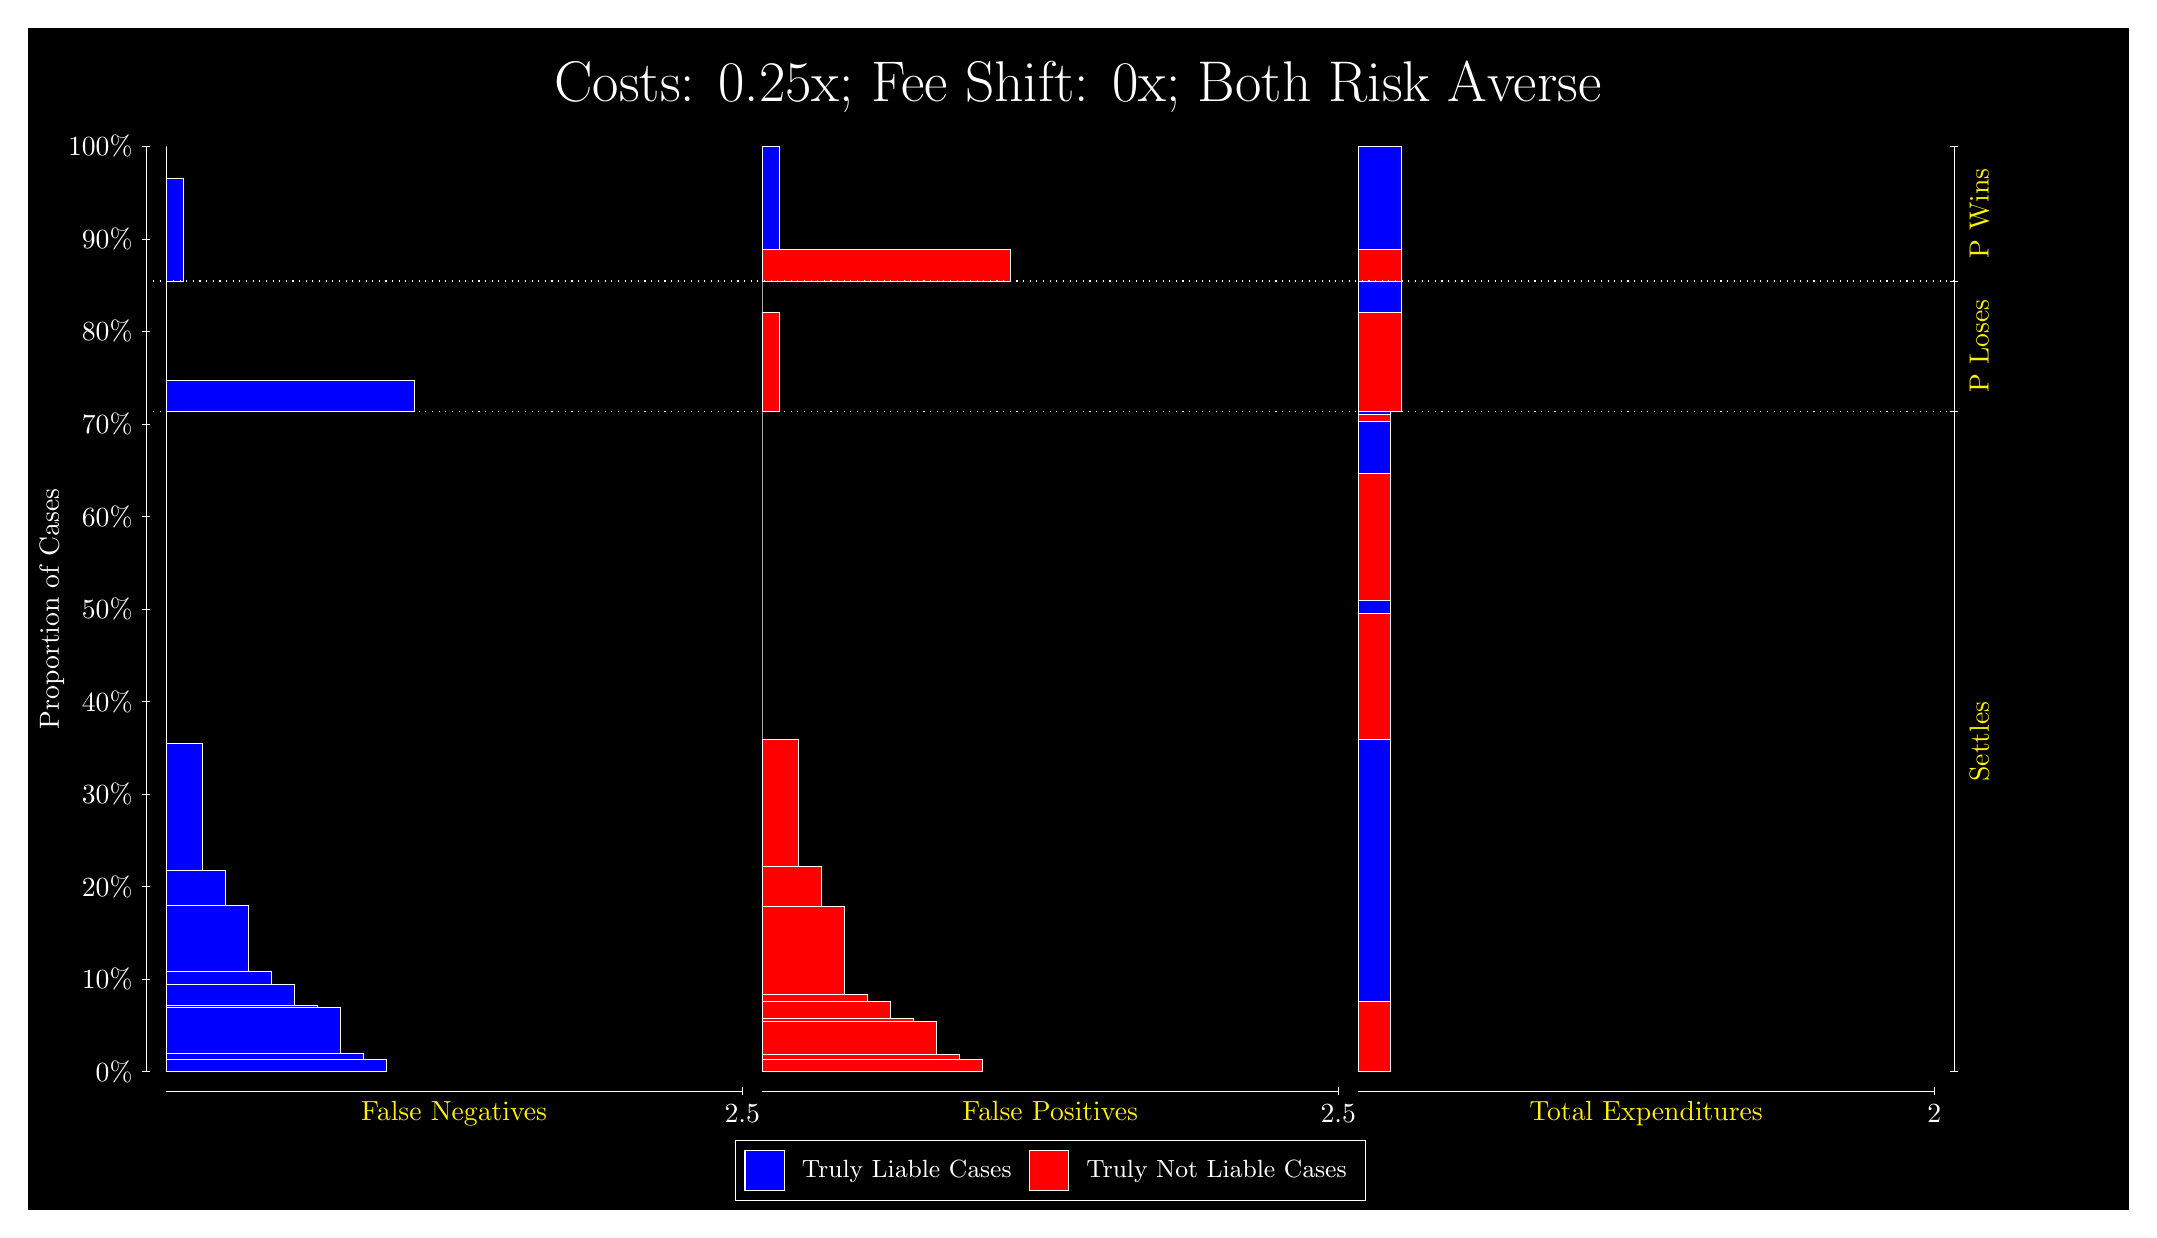
\begin{tikzpicture}
\draw[fill=black] (0,0) rectangle (26.667,15);
\draw[text=white] (0,13.5) rectangle (26.667,15) node[midway] {\huge Costs: 0.25x; Fee Shift: 0x; Both Risk Averse};
\draw[white, very thin] (1.5,1.75) -- (1.5,13.5);
\node[rotate=90, text=white, anchor=center] at (0.3, 7.625) {Proportion of Cases};
\draw[white, very thin] (1.45,1.75) -- (1.55,1.75);
\node[text=white, anchor=east] at (1.45, 1.75) {0\%};
\draw[white, very thin] (1.45,2.925) -- (1.55,2.925);
\node[text=white, anchor=east] at (1.45, 2.925) {10\%};
\draw[white, very thin] (1.45,4.1) -- (1.55,4.1);
\node[text=white, anchor=east] at (1.45, 4.1) {20\%};
\draw[white, very thin] (1.45,5.275) -- (1.55,5.275);
\node[text=white, anchor=east] at (1.45, 5.275) {30\%};
\draw[white, very thin] (1.45,6.45) -- (1.55,6.45);
\node[text=white, anchor=east] at (1.45, 6.45) {40\%};
\draw[white, very thin] (1.45,7.625) -- (1.55,7.625);
\node[text=white, anchor=east] at (1.45, 7.625) {50\%};
\draw[white, very thin] (1.45,8.8) -- (1.55,8.8);
\node[text=white, anchor=east] at (1.45, 8.8) {60\%};
\draw[white, very thin] (1.45,9.975) -- (1.55,9.975);
\node[text=white, anchor=east] at (1.45, 9.975) {70\%};
\draw[white, very thin] (1.45,11.15) -- (1.55,11.15);
\node[text=white, anchor=east] at (1.45, 11.15) {80\%};
\draw[white, very thin] (1.45,12.325) -- (1.55,12.325);
\node[text=white, anchor=east] at (1.45, 12.325) {90\%};
\draw[white, very thin] (1.45,13.5) -- (1.55,13.5);
\node[text=white, anchor=east] at (1.45, 13.5) {100\%};

\draw[white, very thin] (24.457,1.75) -- (24.457,13.5);
\draw[white, very thin] (24.407,1.75) -- (24.507,1.75);
\node[anchor=west] at (24.407, 1.75) {};
\draw[white, very thin] (24.407,10.13) -- (24.507,10.13);
\node[anchor=west] at (24.407, 10.13) {};
\draw[white, very thin] (24.407,11.789) -- (24.507,11.789);
\node[anchor=west] at (24.407, 11.789) {};
\draw[white, very thin] (24.407,13.5) -- (24.507,13.5);
\node[anchor=west] at (24.407, 13.5) {};

\draw[white, very thin, fill=blue] (1.75,1.75) rectangle (4.5495,1.905);
\draw[white, very thin, fill=blue] (1.75,1.905) rectangle (4.2567,1.9785);
\draw[white, very thin, fill=blue] (1.75,1.9785) rectangle (3.964,2.5617);
\draw[white, very thin, fill=blue] (1.75,2.5617) rectangle (3.6712,2.5894);
\draw[white, very thin, fill=blue] (1.75,2.5894) rectangle (3.3784,2.8555);
\draw[white, very thin, fill=blue] (1.75,2.8555) rectangle (3.0857,3.0213);
\draw[white, very thin, fill=blue] (1.75,3.0213) rectangle (2.7929,3.867);
\draw[white, very thin, fill=blue] (1.75,3.867) rectangle (2.5002,4.303);
\draw[white, very thin, fill=blue] (1.75,4.303) rectangle (2.2074,5.9144);
\draw[white, very thin, fill=red] (1.75,5.9144) rectangle (1.75,10.13);
\draw[white, very thin, fill=blue] (1.75,10.13) rectangle (4.8971,10.53);
\draw[white, very thin, fill=red] (1.75,10.53) rectangle (1.75,11.789);
\draw[white, very thin, fill=blue] (1.75,11.789) rectangle (1.9696,13.1);
\draw[white, very thin, fill=red] (1.75,13.1) rectangle (1.75,13.5);
\draw[white, very thin, fill=red] (9.3189,1.75) rectangle (12.118,1.905);
\draw[white, very thin, fill=red] (9.3189,1.905) rectangle (11.826,1.9642);
\draw[white, very thin, fill=red] (9.3189,1.9642) rectangle (11.533,2.3828);
\draw[white, very thin, fill=red] (9.3189,2.3828) rectangle (11.24,2.4248);
\draw[white, very thin, fill=red] (9.3189,2.4248) rectangle (10.947,2.6396);
\draw[white, very thin, fill=red] (9.3189,2.6396) rectangle (10.655,2.7373);
\draw[white, very thin, fill=red] (9.3189,2.7373) rectangle (10.362,3.8503);
\draw[white, very thin, fill=red] (9.3189,3.8503) rectangle (10.069,4.3544);
\draw[white, very thin, fill=red] (9.3189,4.3544) rectangle (9.7763,5.9658);
\draw[white, very thin, fill=blue] (9.3189,5.9658) rectangle (9.3189,10.13);
\draw[white, very thin, fill=red] (9.3189,10.13) rectangle (9.5384,11.389);
\draw[white, very thin, fill=blue] (9.3189,11.389) rectangle (9.3189,11.789);
\draw[white, very thin, fill=red] (9.3189,11.789) rectangle (12.466,12.189);
\draw[white, very thin, fill=blue] (9.3189,12.189) rectangle (9.5384,13.5);
\draw[white, very thin, fill=red] (16.888,1.75) rectangle (17.299,2.6396);
\draw[white, very thin, fill=blue] (16.888,2.6396) rectangle (17.299,5.9645);
\draw[white, very thin, fill=red] (16.888,5.9645) rectangle (17.299,7.5759);
\draw[white, very thin, fill=blue] (16.888,7.5759) rectangle (17.299,7.7309);
\draw[white, very thin, fill=red] (16.888,7.7309) rectangle (17.299,9.348);
\draw[white, very thin, fill=blue] (16.888,9.348) rectangle (17.299,10.005);
\draw[white, very thin, fill=red] (16.888,10.005) rectangle (17.299,10.102);
\draw[white, very thin, fill=blue] (16.888,10.102) rectangle (17.299,10.13);
\draw[white, very thin, fill=red] (16.888,10.13) rectangle (17.437,11.389);
\draw[white, very thin, fill=blue] (16.888,11.389) rectangle (17.437,11.789);
\draw[white, very thin, fill=red] (16.888,11.789) rectangle (17.437,12.189);
\draw[white, very thin, fill=blue] (16.888,12.189) rectangle (17.437,13.5);
\draw[white, dotted] (1.5,10.13) -- (24.457,10.13);
\draw[white, dotted] (1.5,11.789) -- (24.457,11.789);
\draw[white, very thin] (1.75,1.5) -- (9.0689,1.5);
\node[text=yellow, anchor=north] at (5.4094, 1.5) {False Negatives};
\draw[white, very thin] (9.0689,1.45) -- (9.0689,1.55);
\node[text=white, anchor=north] at (9.0689, 1.45) {2.5};

\draw[white, very thin] (9.3189,1.5) -- (16.638,1.5);
\node[text=yellow, anchor=north] at (12.978, 1.5) {False Positives};
\draw[white, very thin] (16.638,1.45) -- (16.638,1.55);
\node[text=white, anchor=north] at (16.638, 1.45) {2.5};

\draw[white, very thin] (16.888,1.5) -- (24.207,1.5);
\node[text=yellow, anchor=north] at (20.547, 1.5) {Total Expenditures};
\draw[white, very thin] (24.207,1.45) -- (24.207,1.55);
\node[text=white, anchor=north] at (24.207, 1.45) {2};

\node[text=yellow, centered, rotate=90] at (24.777, 5.9401) {Settles};
\node[text=yellow, centered, rotate=90] at (24.777, 10.96) {P Loses};
\node[text=yellow, centered, rotate=90] at (24.777, 12.645) {P Wins};

\draw (12.978300999999998,1.5) node[draw=none] (baseCoordinate) {};
\begin{scope}[align=center]
        \matrix[scale=0.5, draw=white, below=0.5cm of baseCoordinate, nodes={draw}, column sep=0.1cm]{
            \node[rectangle, draw, minimum width=0.5cm, minimum height=0.5cm, fill=blue] {}; &
            \node[draw=none, font=\small, text=white] (B) {Truly Liable Cases}; &
            \node[rectangle, draw, minimum width=0.5cm, minimum height=0.5cm, fill=red] {}; &
            \node[draw=none, font=\small, text=white] (B) {Truly Not Liable Cases}; \\
            };
\end{scope}

\end{tikzpicture}
\end{document}